\begin{document}
 %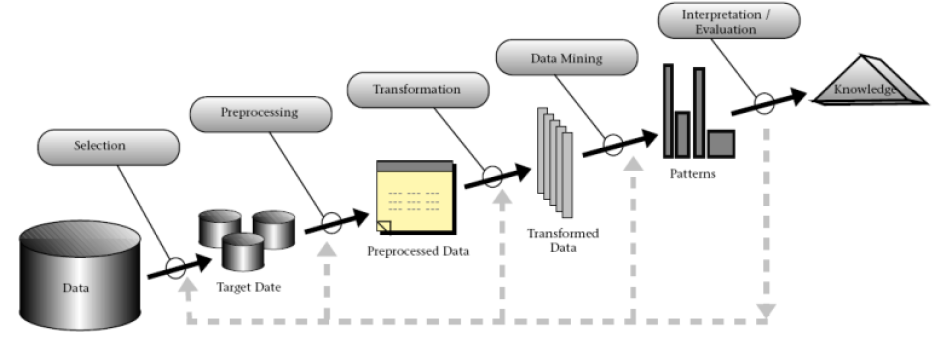
\includegraphics[scale = 0.6]{images/datamining_process.png}\\
 
 
 \begin{center}
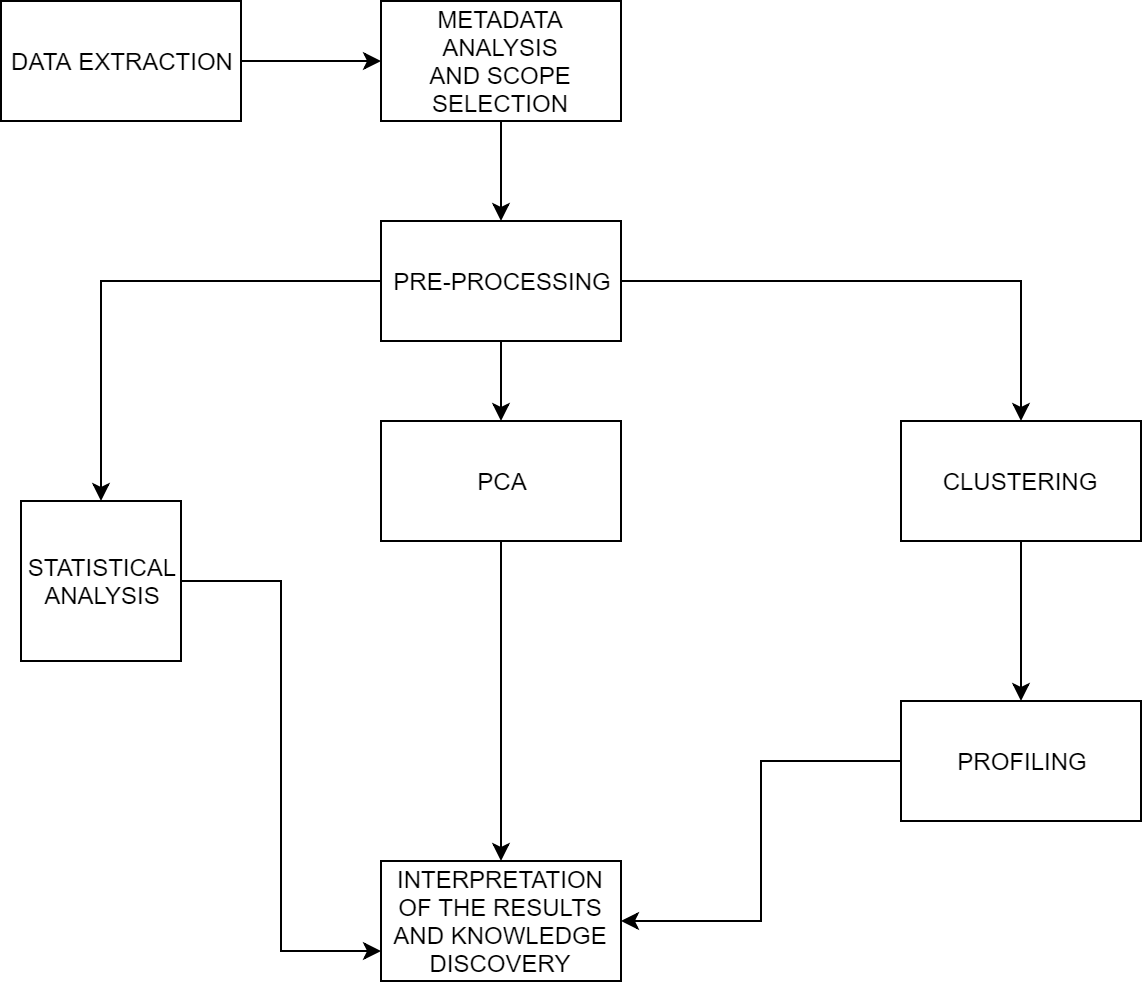
\includegraphics[width=5in]{images/data_process3.png}
\captionof{figure}{Data mining process chart.}
\label{fig:aLabelForReferencing}
\end{center}

%Our data mining process involved the following steps:
\begin{itemize}
    \item Data extraction: obtaining the dataset via Kaggle.
    \item Metadata analysis and scope selection: inspecting the dataset, trying to understand what columns and rows mean and finally constructing the metadata table.
    \item Pre-processing: selecting columns and rows, cleaning the dataset and imputing missing values.
    \item Basic statistical analysis: getting basic statistical indicators and performing some early visualizations of the data.
    \item PCA: decomposing the numerical variables in the principal components (factorial analysis) and projecting the data cloud.
    \item Clustering: dividing the data into different groups by applying hierarchical clustering techniques.
    \item Profiling: detailing the common features of the different clusters.
    \item Interpretation and knowledge discovery: trying to answer our initial question with the results of the different techniques. Performing knowledge extraction based on the previous steps.
\end{itemize}
 
 \begin{comment}
 \begin{itemize}
    \item Selection:
     Once we had understood the meaning of all data with the help of kaggle key sheet we proceeded to do a data selection based on our study scope.\\
    \item Preprocessing:
    In this step we studied and cleaned our original dataset in order to avoid outliners that could affect our final results, also aiming to make data more understandable we created a new derived attribute. \\
    \item Transformation: After having our final dataset we convert our numerical variables  convert into a set of values of linearly uncorrelated variables called principal components(PCA analysis). \\
    \item Data mining: In this step we applied different data mining functions, in order to find patterns among variables which provided us a more understandable vision of the data and the relation between variables.
    \item Interpretation: Once we had our patterns defined, we tried to find answer to our initial answer: What  attributes  influence the selection of a romantic partner? \\
\end{itemize}
\end{comment}
 
\end{document}